% ============================================================================
% QCD: quark-quark scattering by one-gluon exchange, lowest order
%        q_i(p,s) + q'_k(k,r)  ->  q_j(p',s') + q'_l(k',r')        (two different flavours)
% The QCD analogue of the e-mu diagram: same layout; first quark q blue, second quark q' red, gluon = black coil.
%
% Conventions as in qcd_rules.tex (Feynman gauge, D_mu = d_mu - i g A^a_mu t^a):
%   quark-gluon vertex   i g gamma^mu t^a_{ji}   (j = outgoing colour, i = incoming colour)
%   gluon propagator     -i g_{mu nu} delta^{ab} / (q^2 + i eps)
% Colour indices: quarks i,j,k,l = 1..3 ; gluon a,b = 1..8.
% Page = PowerPoint widescreen (13.333in x 7.5in).  Compile with pdflatex or lualatex.
% ============================================================================
\documentclass[10pt]{article}
\usepackage{lmodern}
\usepackage[T1]{fontenc}
\usepackage{amsmath,amssymb}
\usepackage{xcolor}
\usepackage{graphicx}
\usepackage{tikz}
\usetikzlibrary{decorations.markings,decorations.pathmorphing,arrows.meta,positioning}
\usepackage[paperwidth=338.67mm,paperheight=190.5mm,
            left=5mm,right=5mm,top=3mm,bottom=3mm]{geometry}
\pagestyle{empty}
\setlength{\parindent}{0pt}

\definecolor{qcol}{HTML}{1F4E9C}   % first quark q  (same blue as the electron / the QCD rules page)
\definecolor{rcol}{HTML}{C0392B}   % second quark q' (same red as the muon)

\tikzset{
  bf/.style={line width=2.4pt,                               % quark line with arrow
    decoration={markings,
      mark=at position 0.55 with {\arrow{Stealth[length=4.4mm,width=3.6mm]}}},
    postaction={decorate}},
  bmom/.style={-{Stealth[length=2.8mm,width=2.3mm]},line width=1pt,color=black!70},
  qlab/.style={font=\fontsize{30}{34}\selectfont,text=qcol,inner sep=2pt},
  rlab/.style={font=\fontsize{30}{34}\selectfont,text=rcol,inner sep=2pt},
  plab/.style={font=\fontsize{28}{32}\selectfont,inner sep=2pt},
  qvbox/.style={font=\fontsize{30}{34}\selectfont,text=qcol,draw=qcol,fill=qcol!8,
                line width=1.2pt,rounded corners=4pt,inner sep=7pt},
  rvbox/.style={font=\fontsize{30}{34}\selectfont,text=rcol,draw=rcol,fill=rcol!8,
                line width=1.2pt,rounded corners=4pt,inner sep=7pt},
  pbox/.style={font=\fontsize{30}{34}\selectfont,draw=black!60,fill=black!4,
               line width=1.2pt,rounded corners=4pt,inner sep=8pt},
}

\begin{document}
\vspace*{\fill}
\centering
\scalebox{1.22}{%
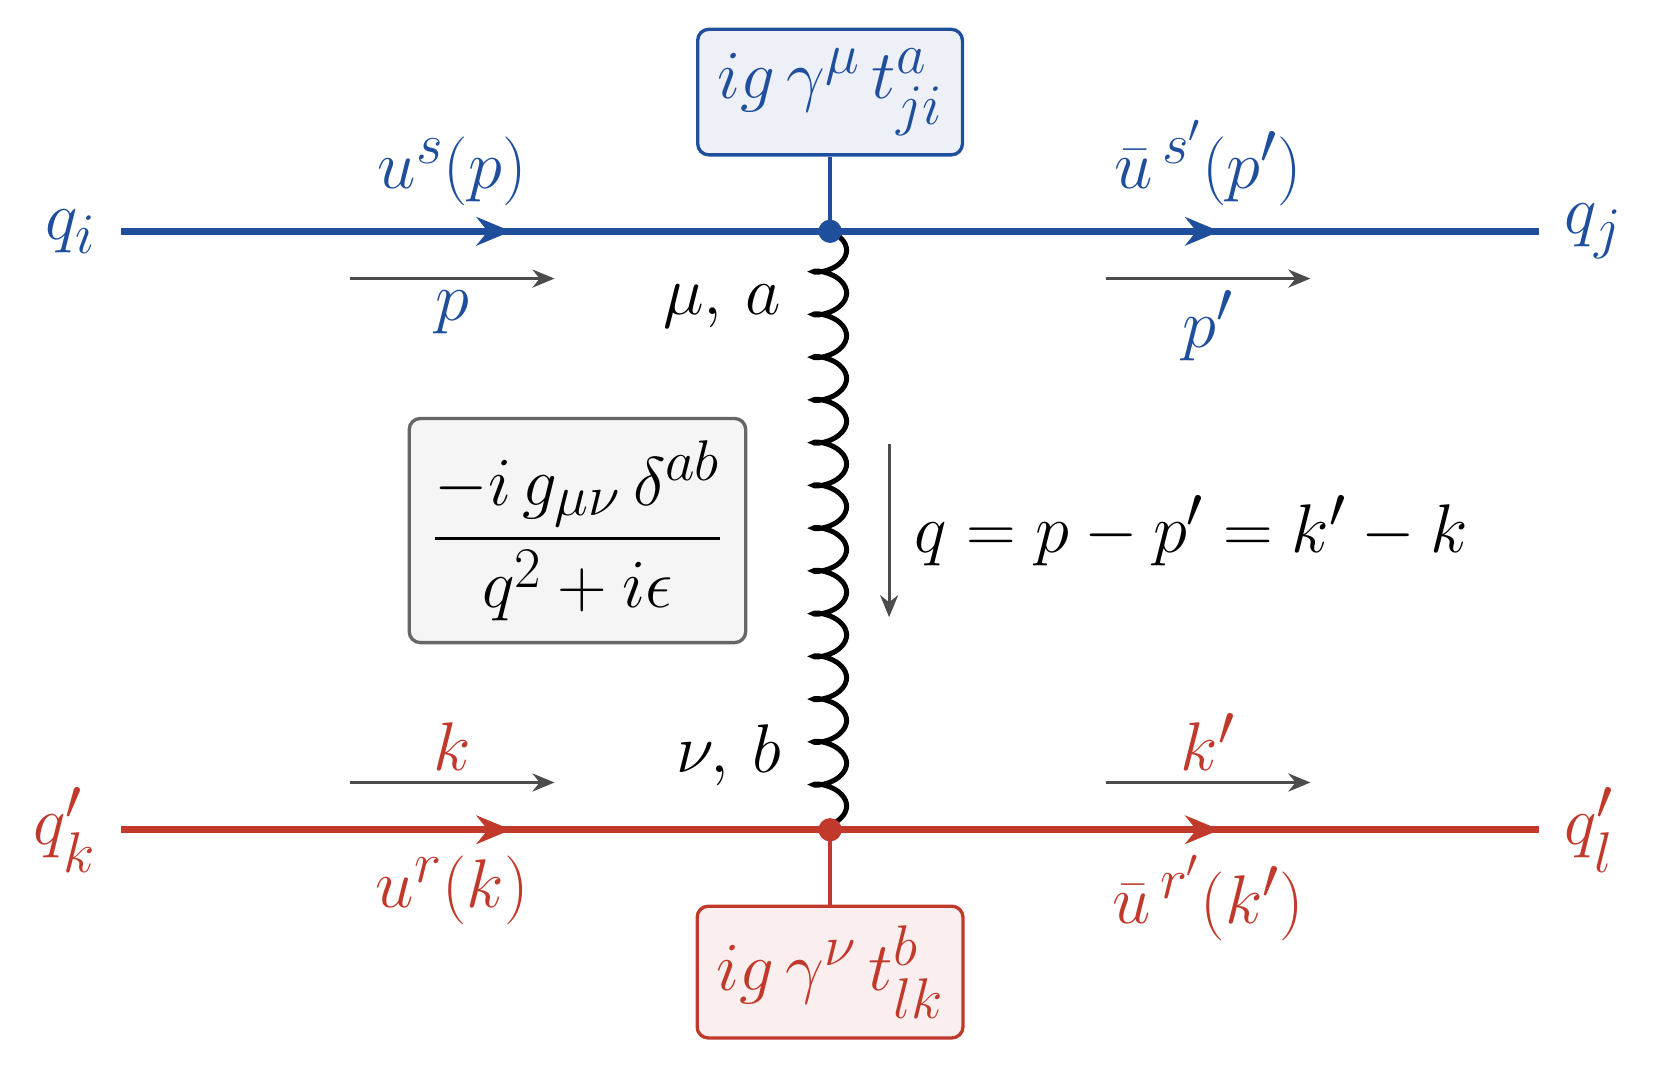
\begin{tikzpicture}[x=1cm,y=1cm]
  % whole number of coils on the gluon (14 coils over 7.6 cm): no kinks at the vertices
  \pgfmathsetlengthmacro{\sgl}{7.6cm/14}
  % ----------------------------------------------------------- quark lines
  \draw[bf,color=qcol] (-9,3.8) -- (0,3.8);            % incoming quark q
  \draw[bf,color=qcol] ( 0,3.8) -- (9,3.8);            % outgoing quark q
  \draw[bf,color=rcol] (-9,-3.8) -- (0,-3.8);          % incoming quark q'
  \draw[bf,color=rcol] ( 0,-3.8) -- (9,-3.8);          % outgoing quark q'

  % ----------------------------------------------------------- gluon (black coil)
  \draw[line width=1.8pt,decorate,
        decoration={coil,aspect=0.5,segment length=\sgl,amplitude=2.1mm}] (0,3.8) -- (0,-3.8);

  % ----------------------------------------------------------- vertices (dots + boxed vertex factors)
  \fill[qcol] (0,3.8)  circle (4.2pt);
  \fill[rcol] (0,-3.8) circle (4.2pt);
  \draw[qcol,line width=1.2pt] (0,3.8)  -- (0,4.75);
  \draw[rcol,line width=1.2pt] (0,-3.8) -- (0,-4.75);
  \node[qvbox,anchor=south] at (0,4.75)  {$i g\,\gamma^{\mu}\,t^{a}_{ji}$};
  \node[rvbox,anchor=north] at (0,-4.75) {$i g\,\gamma^{\nu}\,t^{b}_{lk}$};

  % ----------------------------------------------------------- quark names and colour indices at the line ends
  \node[qlab,anchor=east] at (-9.25,3.8)  {$q_{i}$};
  \node[qlab,anchor=west] at ( 9.25,3.8)  {$q_{j}$};
  \node[rlab,anchor=east] at (-9.25,-3.8) {$q'_{k}$};
  \node[rlab,anchor=west] at ( 9.25,-3.8) {$q'_{l}$};

  % ----------------------------------------------------------- external spinors (outside the lines)
  \node[qlab,anchor=south] at (-4.8, 4.05) {$u^{s}(p)$};
  \node[qlab,anchor=south] at ( 4.8, 4.05) {$\bar u^{\,s'}(p')$};
  \node[rlab,anchor=north] at (-4.8,-4.05) {$u^{r}(k)$};
  \node[rlab,anchor=north] at ( 4.8,-4.05) {$\bar u^{\,r'}(k')$};

  % ----------------------------------------------------------- momenta (inside, between the lines)
  \draw[bmom] (-6.1,3.2) -- (-3.5,3.2);  \node[plab,anchor=north,text=qcol] at (-4.8,3.12) {$p$};
  \draw[bmom] ( 3.5,3.2) -- ( 6.1,3.2);  \node[plab,anchor=north,text=qcol] at ( 4.8,3.12) {$p'$};
  \draw[bmom] (-6.1,-3.2) -- (-3.5,-3.2); \node[plab,anchor=south,text=rcol] at (-4.8,-3.12) {$k$};
  \draw[bmom] ( 3.5,-3.2) -- ( 6.1,-3.2); \node[plab,anchor=south,text=rcol] at ( 4.8,-3.12) {$k'$};

  % ----------------------------------------------------------- gluon: indices, momentum, propagator, colour structure
  \node[plab,anchor=east] at (-0.55, 2.85)  {$\mu,\,a$};
  \node[plab,anchor=east] at (-0.55,-2.85)  {$\nu,\,b$};
  \draw[bmom] (0.75,1.1) -- (0.75,-1.1);
  \node[plab,anchor=west] at (1.0,0) {$q=p-p'=k'-k$};
  \node[pbox,anchor=east] at (-1.05,0) {$\displaystyle\frac{-i\,g_{\mu\nu}\,\delta^{ab}}{q^{2}+i\epsilon}$};
\end{tikzpicture}}
\vfill
\end{document}
